%Used template from: https://github.com/jpeisenbarth/SRS-Tex
\documentclass{scrreprt}
\usepackage{listings}
\usepackage{underscore}
\usepackage[bookmarks=true]{hyperref}
\usepackage[utf8]{inputenc}
\usepackage[english]{babel}
\usepackage{graphicx}
\usepackage{usecases}
\graphicspath{ {./images/} }
\hypersetup{
    bookmarks=false,    % show bookmarks bar?
    pdftitle={Software Requirement Specification},    % title
    pdfauthor={Saad Ismail, Shehryar Naeem, Hassan Berry},                     % author
    pdfsubject={TeX and LaTeX},                        % subject of the document
    pdfkeywords={TeX, LaTeX, graphics, images}, % list of keywords
    colorlinks=true,       % false: boxed links; true: colored links
    linkcolor=blue,       % color of internal links
    citecolor=black,       % color of links to bibliography
    filecolor=black,        % color of file links
    urlcolor=purple,        % color of external links
    linktoc=page            % only page is linked
}%
\def\myversion{1.0 }
\date{}
%\title
\usepackage{hyperref}
\begin{document}

\begin{flushright}
    \rule{16cm}{5pt}\vskip1cm
    \begin{bfseries}
        \Huge{SOFTWARE REQUIREMENTS\\ SPECIFICATION}\\
        \vspace{1.9cm}
        for\\
        \vspace{1.9cm}
        Crowd Fund Raising\\
        \vspace{1.9cm}
        Prepared by\\Shehryar Naeem, Hassan Berry, Saad Ismail\\
        \vspace{1.9cm}
        FAST-NUCES Karachi\\
        \vspace{1.9cm}
        \today\\
    \end{bfseries}
\end{flushright}

\tableofcontents


\chapter*{Revision History}

\begin{center}
    \begin{tabular}{|c|c|c|c|}
        \hline
	    Name & Date & Reason For Changes & Version\\
        \hline
	    Hassan Berry & 19-11-2018 & Initially document created & 1\\
        \hline
	    Shehryar Naeem & 20-11-2018 & Usecase Diagram & 2\\
        \hline
        Hassan Berry & 21-11-2018 & Proof-read & 3\\
        \hline
        Shehryar Naeem & 22-11-2018 & Dressed Usecases & 4\\
        \hline
        Saad Ismail & 22-11-2018 & docx to latex conversion & 5\\
        \hline
        Saad Ismail & 22-11-2018 & Last minute changes & 6\\
        \hline
    \end{tabular}
\end{center}

\chapter*{Distribution List}

\begin{center}
    \begin{tabular}{|c|c|}
        \hline
	    Name & Role\\
        \hline
	    Ms. Rubab Jaffar & Supervisor\\
        \hline
	    Mr. Awais Ahmed & Co-Supervisor\\
        \hline
    \end{tabular}
\end{center}

\chapter{Introduction}

\section{Purpose}
To provide a detailed \textbf{overview} of our software product, its parameters and goals. This document describes the project's target audience and its user \textbf{interface}, hardware and software requirements.

\section{Document Conventions}
Latex document class: scrreprt

\section{Intended Audience and Reading Suggestions}
Supervisors, and team members.

\section{References}
Not applicable.


\chapter{Overall Description}

\section{Product Perspective}
This is a new self-contained product.

\section{Background}
The background of this project is the severe need of a consolidated platform which combines crowd-funding, crowd-sourcing and provides a platform for people interested in philanthropic and social services.

\section{Project Scope}
This project will consist of creating a marketable, and deploy-able application based on the concept of crowd-sourcing and crowd-funding. The modules of the project will in include a mobile application and web based front end where users can interact with the database.

\subsection{Deliverables}
\begin{itemize}
  \item Functional Database
  \item Web based application
\end{itemize}

\subsection{Out of Scope}
\begin{itemize}
  \item Dynamic Website
  \item Mobile Application
\end{itemize}

\section{Project Objectives}
The objective of this project to solve the problem of having a consolidated platform where crowd-sourcing and crowd-funding is combined to be a ‘one-stop’ place for people seeking funds, companies/individuals looking to invest in great ideas, and individuals/organizations looking to form a team for a specific project.

\section{Stakeholders}
\begin{enumerate}
  \item Users
  \item Administrators
\end{enumerate}

\section{Operating Environment}
The project can be hosted on any PC platforms, regardless of architecture and operating system being used. The development, testing and official support is only for Intel based CPU with Linux Operating System.

\section{System Constraints}
\begin{itemize}
  \item In order to implement payment system, we will have to partnership with local and international banks.
  \item The system is open to spam, we are totally dependent on end-users to reduce spam.
\end{itemize}

\section{Assumptions and Dependencies}
We are totally dependent on banks to handle payments to the projects and we will have to transfer payments manually to the end-users.

\chapter{External Interface Requirements}

\section{User Interfaces}
We will provide user-friendly, responsive and easy to use web interfaces for our customers. Those will be based on Bootstrap v4.

\section{Software Interfaces}
There are three main components of the product.

\begin{enumerate}
    \item \textbf{Front-end}\\
        Powered by Angular 2 (TypeScript)
    \item \textbf{Back-end}\\
        Powered by Node.JS and Express.JS
    \item \textbf{Database}\\
        Powered by MySQL
\end{enumerate}

\section{Hardware Interfaces}
For initial release, the product will run on a single node but in future, the three software components can be deployed on different nodes to increase concurrency and optimizing the page load speed.

\section{Communications Interfaces}
\begin{itemize}
    \item HTTP(s) (80, 443)
    \item MySQL (3306)
    \item SMTP (465 - only outgoing)
\end{itemize}

\chapter{Functional Requirements}

\section{Functional Hierarchy}

\begin{enumerate}
    \item Register
        \begin{itemize}
            \item Enter User Information
            \item Account Verification
        \end{itemize}
    \item Login
        \begin{itemize}
            \item Enter Credentials
            \item Authenticate and Redirect to related Webpage
        \end{itemize}
    \item Initiate New Project
        \begin{itemize}
            \item Enter Description and Milestones
            \item Select Related Category
        \end{itemize}
    \item Send Funds (Mocked)
        \begin{itemize}
            \item Project Selection
            \item Select Fund Type
            \item Send Funds
            \item Authorize and Confirm Transaction
        \end{itemize}
    \item Vote projects
\end{enumerate}

\section{Use cases}

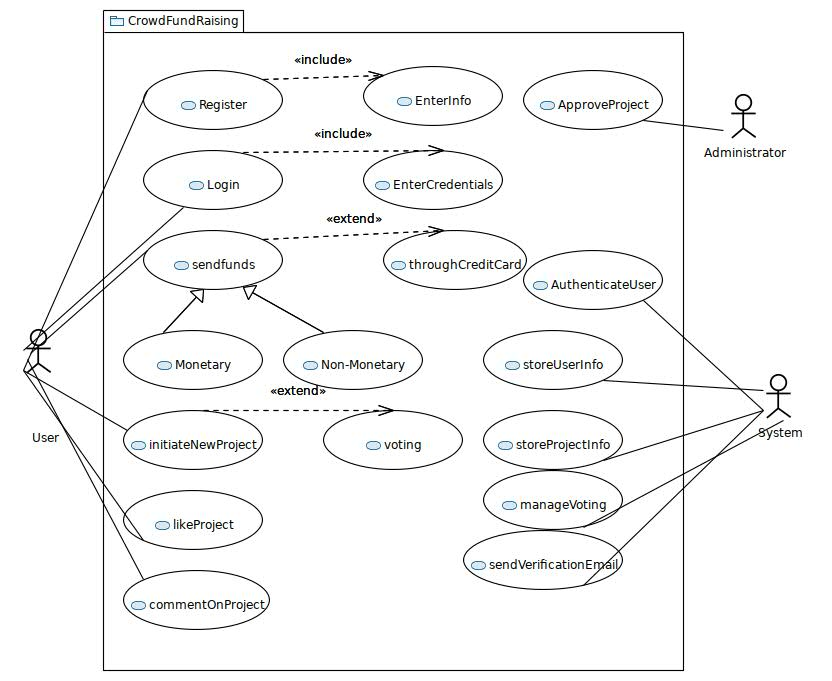
\includegraphics[width=\textwidth]{usecase-diagram.jpeg}
\newpage

\begin{usecase}
    \addtitle{Use Case 1}{Login}
    \addfield{Primary Actor:}{End-User}
    \additemizedfield{Preconditions:}{
        \item User is already registered.
    }
    \additemizedfield{Postconditions:}{
        \item The user can view his/her profile and can access other features.
    }
    \addscenario{Main Success Scenario:}{
	    \item Enter email
	    \item Enter password
	    \item Authenticate
    }
    \addscenario{Alternate Scenarios:}{
    	\item[1.a] Invalid login details:
    		\begin{enumerate}
    		\item[1.] System shows failure message
    		\end{enumerate}
    }
\end{usecase}
\newpage

\begin{usecase}
    \addtitle{Use Case 2}{Register}
    \addfield{Primary Actor:}{End-User}
    \additemizedfield{Preconditions:}{
        \item User is not already registered.
    }
    \additemizedfield{Postconditions:}{
        \item The user can login using his/her account.
    }
    \addscenario{Main Success Scenario:}{
        \item Enter fullname
	    \item Enter email
	    \item Enter password
	    \item Enter confirm password
	    \item System registers the users and sends verification email.
	    \item User verifies the account by clicking the link received in the email.
    }
    \addscenario{Alternate Scenarios:}{
    	\item[1.a] User not verified:
    		\begin{enumerate}
    		\item[1.] User will not be allowed to post new projects/vote on existing projects.
    		\end{enumerate}
    }
\end{usecase}
\newpage

\begin{usecase}
    \addtitle{Use Case 3}{Send Funds}
    \addfield{Primary Actor:}{End-User}
    \additemizedfield{Preconditions:}{
        \item User is already logged in.
    }
    \additemizedfield{Postconditions:}{
        \item The funds will be scheduled to be sent.
    }
    \addscenario{Main Success Scenario:}{
	    \item Enter amount
	    \item Confirm
    }
    \addscenario{Alternate Scenarios:}{
    	\item[1.a] Amount not valid:
    		\begin{enumerate}
    		\item[1.] System shows failure message.
    		\item[2.] Transaction is cancelled.
    		\end{enumerate}
    }
\end{usecase}
\newpage

\begin{usecase}
    \addtitle{Use Case 4}{Create New Project}
    \addfield{Primary Actor:}{End-User}
    \additemizedfield{Preconditions:}{
        \item User is already logged in.
    }
    \additemizedfield{Postconditions:}{
        \item The project stored in the database and available to vote.
    }
    \addscenario{Main Success Scenario:}{
	    \item Enter project details
	    \item Enter milestones
	    \item Confirm
    }
\end{usecase}
\newpage

\begin{usecase}
    \addtitle{Use Case 5}{Approve Project}
    \addfield{Primary Actor:}{Administrator}
    \additemizedfield{Preconditions:}{
        \item The project should have reached the voting milestone.
    }
    \additemizedfield{Postconditions:}{
        \item The new project will be included in the category.
    }
    \addscenario{Main Success Scenario:}{
        \item Verify project details and users authenticity
	    \item Put the project in suitable category.
    }
    \addscenario{Alternate Scenarios:}{
    	\item[1.a] Project not suitable:
    		\begin{enumerate}
    		\item[1.] Delete the project.
    		\end{enumerate}
    }
\end{usecase}
\newpage

\begin{usecase}
    \addtitle{Use Case 6}{Authenticate User}
    \addfield{Secondary Actor:}{System}
    \additemizedfield{Preconditions:}{
        \item User is not already logged in.
    }
    \additemizedfield{Postconditions:}{
        \item The user can view his/her profile and can access other features.
    }
    \addscenario{Main Success Scenario:}{
	    \item Verify user details
	    \item Redirect user to suitable webpage
    }
    \addscenario{Alternate Scenarios:}{
        \item[1.a] Account details incorrect:
    		\begin{enumerate}
    		\item[1.] System shows failure message
    		\end{enumerate}
    	\item[2.a] Account not verified:
    		\begin{enumerate}
    		\item[1.] System shows warning message
    		\end{enumerate}
    	
    }
\end{usecase}
\newpage

\chapter{Other Nonfunctional Requirements}

\section{Performance Requirements}
The project must be easily accessible and fast to the end-users. The page load time must be less than 10 seconds, even on slow internet connections. The interface must be user friendly and easy to use so that the user doesn't have any confusion or difficulty. The page rank of the website must be prepared according to the Google Page Rank Algorithm which will allow it to show up easily in Google Search Results.

\section{Safety Requirements}
Users, their payment information and other sensitive information must be handled safely. Moreover, the use of bots must be eliminated and great care will be taken to ensure that the personal details of the Users are not compromised in any way.\\\\ A two factor authentication system can be utilized to ensure that the login security of users is protected and no malicious attack will be made successful.

\section{Security Requirements}
The product must not be vulnerable to any known issues and other security bugs like SQL injection, XSS etc.\\\\The possibility of bots forming usernames and accounts must be eliminated and to do this, we will utilize Google Recaptcha which will ensure that the user is a human being. 

\section{Software Quality Attributes}
Code quality must be up-to the mark. Unit and Integration tests should be written after the initial release.\\\\All the stages of the Software Development Life Cycle must be followed. Moreover homogenization must be done in order to add clarity and consistency to our models and ensuring that all the stake holders clearly follow the process and can check that their requirements are being followed.

\end{document}